\chapter{The Standard Model and Its Future}\label{sec:theory}
In Section \ref{sec:introduction}, we introduced the few obstacles facing the SM: The existence of dark matter, baryon-antibaryon asymmetry, and the evidence of neutrino masses and mixing.
The SM Lagrangian, written as in formula \ref{eq:SM}, does not have particle fields that can explain those phenomena.
\begin{equation}
\label{eq:SM}
\mathcal{L}_{SM} = \mathcal{L}_{Higgs}+\mathcal{L}_{Gauge}+\mathcal{L}_{Kinetic}+\mathcal{L}_{Yukawa}
\end{equation}
Since it can not be explained by any of the particles' fields in the SM, it requires the addition of new particles' fields or new terms in the current SM Lagrangian expression.
New terms in the SM Lagrangian entail new vertices in the Feynman diagram, which open the door for a new understanding of high energy physics.
However, if those observations did not exist, the SM is complete within its framework except for the naturalness problem.
The naturalness problem originates from the SM Higgs being a scalar particle.
The formula \ref{eq:SM} has three fields: boson, fermion, and scalar.
\section{The Standard Model}
\subsection{Fermion sector}

Quantum Field Theory (QFT), humanity's mathematical framework used for the SM, explains matter as an excited state of fermion fields derived from the canonical quantization of the SM Lagrangian's fermion fields.
%Also, QFT explains forces of the universe as the exchange of boson particles among the fermions, which can be derived from the fermion kinetic term of the SM Lagrangian.
The fermions' fields have baryon symmetry, and slightly broken isospin, and chiral symmetries in the SM Lagrangian.
Baryon symmetry is evident in $\mathcal{L}_{Kinetic}$ and $\mathcal{L}_{Yukawa}$ of formula \ref{eq:SM}. 
Formula \ref{eq:Bar1} and \ref{eq:Bar2} shows $\mathcal{L}_{Kinetic}$ and $\mathcal{L}_{Yukawa}$ Lagrangian terms' expanded forms for different chriality and up-type and down-type fermions.
\begin{equation}
\label{eq:Bar1}
	\mathcal{L}_{Kinetic}  = \bar{Q_{L}}\cdot i\gamma^{\mu}D_{\mu}Q_{L}+\bar{d_{R}}\cdot i\gamma^{\mu}D_{\mu}d_{R}+\bar{u_{R}}\cdot i\gamma^{\mu}D_{\mu}u_{R}+h.c\;(Hermitian\;Conjugate).
\end{equation}

\begin{equation}
\label{eq:Bar2}
	\mathcal{L}_{Yukawa}  = \bar{Q_{L}}\cdot Y^{d}_{ij}H\cdot d_{R}+\bar{Q_{L}}^{*}\cdot Y^{u}_{ij}H^{*}\cdot u_{R}+h.c\;(Hermitian\;Conjugate).
\end{equation}
In formular \ref{eq:Bar1}, Dirac matrices are summed up over Lorentz indices for Lorentz invariance. 
In formula \ref{eq:Bar1} and \ref{eq:Bar2}, $d_{R}$, $u_{R}$ are right-hand fermions for down-type ($\ell$ for leptons) and up-type (\PGnl for leptons) fermions respectively.
$Q_{L}$ is a left-hand fermion doublet as expressed in formula \ref{eq:Bar3}.
\begin{equation}
\label{eq:Bar3}
	Q_{L}=\begin{bmatrix}
	u_L \\
	d_L \\
\end{bmatrix}
\end{equation}
Since fermions with left-hand chirality behave differently from fermions with right-hand chirality,
the covariant derivatives are also different for left-hand kinetic term and right-hand kinetic terms, being defined in the formula \ref{eq:covld} and in \ref{eq:covrd}.
\begin{equation}
\label{eq:covld}
	D_{\mu}  = i\partial_{\mu}-\frac{1}{2}g\mathcal{T}\cdot W_{\mu}-\frac{1}{2}g^{'}YB_{\mu} 
\end{equation}
\begin{equation}
\label{eq:covrd}
	D_{\mu}  = i\partial_{\mu}-\frac{1}{2}g^{'}YB_{\mu} 
\end{equation}
$\mathcal{T}$ is isospin for SU(2) weak force, and \Pg, W are couplings and fields for the weak theory. \Pg' and B are respective variables for quantum electrodynamics (QED).
As a fermion transforms as in formula \ref{eq:Bar4}, we can see all the terms in the formula \ref{eq:Bar1} and \ref{eq:Bar2} are invariant. 
\begin{equation}
\label{eq:Bar4}
	q \to q\cdot e^{i\alpha_{B}} .
\end{equation}
Thus, fermion sector of the SM Lagrangian satisfies the baryon symmetry. 


The SM's weak force satisfies the Special unitary group, SU(2) symmetry.
Isospin is the quantum number for the SU(2) symmetry of the SM.
Up-type fermions and down-type fermions have ($\frac{1}{2}$,$\frac{-1}{2}$) isospin values in the SM.
If the isospin symmetry were perfect in the SM, it could have many implications for baryons and others in the universe.
Baryons of protons and neutrons consist of 3 quark fermions: (u,u,d) and (u,d,d) respectively.
As SU(2) group generator transits the isospin quantum number from up-type to down-type, proton and neutron would have the same mass if up quark and down quark had same masees.
However, up quark and down quark have different masses.
Thus, the isospin symmetry is slightly broken in the SM and result in slight difference in mass of protons and neutrons.

The SM fermions also have chiral symmetry breaking.
Fermions can transform under chiral rotation as given in formular \ref{eq:Chi1}. 
\begin{equation}
\label{eq:Chi1}
\begin{bmatrix}	u_L' \\	d_L' \\\end{bmatrix}
	=e^{i\alpha_5}\cdot 
\begin{bmatrix} u_L' \\ d_L' \\\end{bmatrix}, \;
u_R' = e^{-i\alpha_5}\cdot u_R, \; 
d_R' = e^{-i\alpha_5}\cdot d_R, \; 
\end{equation}
Transformation phase is in opposite direction for left-hand and right-hand fermions.
Under the transformation formular of \ref{eq:Chi1}, the mass of fermions are not always invariant under chiral rotation.
Formular \ref{eq:Chi2} shows the change of fermion's mass under chiral rotation.
\begin{equation}
\label{eq:Chi2}
	m_q\cdot(\bar{u_R'}u_L'+\bar{d_R'}d_L') = m_q\cdot e^{2i\alpha}\cdot (\bar{u_R}u_L+\bar{d_R}d_L)
\end{equation}
The mass is only invariant when the $m_{q}$ = 0.
However, fermions' masses are not zero and the chiral symmetry breaking is proportional to the masses of the fermions.
It results in ``Technical naturalness'' of the SM fermions', which makes quatum correction to be also proportional to the same chiral symmetry breaking.
It provides a significant advantage in QFT's renormalization.
QFT's renormalization understands the observed mass of particles in terms of its bare mass and correction as in \ref{eq:ren}.
\begin{equation}
\label{eq:ren}
	m^{2}=m_{0}^{2}+\delta m^2.
\end{equation}
For fermions, the mass correction term ($\delta m_{f}^2$) is multiplicative to the chiral symmetry breaking as in formular \ref{eq:Chi3}.
\begin{equation}
\label{eq:Chi3}
	\delta m_{f}^2=m_{f}\cdot \frac{g^2}{16\pi^2}\cdot ln\frac{\Lambda}{m_{f}},\;\Lambda = New\;Physics\;Mass\;Scale
\end{equation}
The mass correction term at a new BSM physics scale is multiplied by the chiral symmetry breaking.
Its multiplicative nature protects fermion fields' from extreme radiative correction at BSM scale in the renormalization process.

\subsection{Gauge Sector}
Likewise, the bosons' fields satisfy special QFT framework symmetries.
The boson satisfies the U(1), SU(2), or SU(3) gauge symmetry and is expressed in gauge terms as in formula \ref{eq:Lag2}.
\begin{equation}
\label{eq:Lag2}
	\mathcal{L}_{Gauge} = -\frac{1}{4}B_{\mu\nu}\cdot B^{\mu\nu}-\frac{1}{4}W_{\mu\nu}^{\mathcal{T}}\cdot W^{\mu\nu}_{\mathcal{T}}-\frac{1}{4}G_{\mu\nu}^{\alpha}\cdot G^{\mu\nu}_{\alpha}.
\end{equation}
, where B, W, and G are QED, weak, quantum chromodynamics (QCD) fields, $\mathcal{T}$, $\alpha$ are SU(2), SU(3) group indices, respectively.

Gauge symmetry, like technical naturalness for fermions, also provides one significant advantage for renormalization.
In case of gauge symmetry, the correction term ($\delta m_{f}^2$) of formula \ref{eq:ren} becomes zero and protects boson fields from the divergence of radiative correction in the renormalization process.

\subsection{Scalar Sector}
Unlike fermions or gauge bosons, the scalar field of the Higgs boson is not protected by any symmetry. It is subject to large radiative corrections, especially from the top quark loop.
Thus, the necessary radiative corrections are enormous for the SM to be valid up to the Planck or Grand Unification Theory (GUT) scales of $10^{16}$\GeV.
One needs exorbitant fine-tuning to fit the Higgs mass at the observed value of 125\GeV.
A simple mathematical expression is shown in formular \ref{eq:sca1}
\begin{equation}
\label{eq:sca1}
	125\GeV = m_{0}^{2}-\frac{g^2}{16\pi^2}\cdot\Lambda^{2},\; \Lambda = O(10^{16})	
\end{equation}
One of the most popular solutions to this problem is Supersymmetry (SUSY), which assigns chirality to the Higgs particle.
SUSY solves the fine-tuning problem, neutrino masses, and provides a candidate for DM.

Unfortunately, the LHC has found no significant excess over the SM background in their search for SUSY\cite{SUSY}.
Although the non-observation of supersymmetric partner particles does not invalidate SUSY, it makes it less attractive among the particle physics community.
Non-observation of superpartners, particularly the stop (scalar partner of the top quark), has pushed its mass beyond 1\TeV.
It generates a ``little hierarchy'' problem, but an alternative ``neutral naturalness'' solution remains.

\section{Motivation for Neutral Naturalness}
The top partners are not charged under the SM color group in the framework of neutral naturalness.
Because of being colorless, their production cross section is much smaller, and the present limits on the top SUSY partner particles are well below 1\TeV.
Examples of neutral naturalness models are the Twin Higgs \cite{Chacko:2005pe},
Folded SUSY \cite{Burdman:2006tz}, and the Quirky Little Higgs \cite{Cai:2008au} models.
Twin Higgs realizes the Higgs as a pseudo-Goldstone boson that protect the weak scale from radiative corrections up to scales of order 5 - 10 TeV \cite{Chacko:2005pe}.
Naturalness constrains the masses of most of the twin/mirror partners not to exceed a few hundred\GeV \cite{Chacko:2005pe}.
Twin baryons can constitute some or all of the dark matter in the universe, depending on the baryon asymmetry in the mirror sector. \cite{Chacko:2005pe}.
Thus, Twin Higgs model can solve both the naturalness problem and dark matter issue of the SM.
Folded SUSY postulates that one loop quadratic divergences of the Standard Model Higgs field are cancelled by ``folded partners'', and the gauge quantum numbers for the folded partners are a bit different from conventional SUSY \cite{Burdman:2006tz}.
The familiar squarks and gauginos need not be present \cite{Burdman:2006tz}.
The only folded partners with masses less than 50 \GeV are the gluons of mirror color \cite{Burdman:2006tz}. 
These folded gluons will confine into folded glueballs at a scale of order a few GeV \cite{Burdman:2006tz}.



In the Quirky Little Higgs scenario, there are some new fermions that couple to a new non-Abelian gauge group referred to as ``infracolor'' \cite{Cai:2008au}.
The fermions charged under this new gauge group are called quirks in analogy to the traditional quarks \cite{Cai:2008au}.
The dark top quirk and top quark are related by an SU(6) bulk gauge symmetry in which their respective confining gauge groups are embedded \cite{Cai:2008au}. 
Quirky Little Higgs theorizes that top loop contribution to the Higgs mass is cancelled by an uncolored heavy ``top quirk'' charged under a different SU(3) gauge group \cite{Cai:2008au}. 
The Higgs in this model is a pseudo-Nambu-Goldstone boson and its mass parameter is protected by an $SU(3)_{W}$ symmetry \cite{Cai:2008au}.
Depending on the ``quirk'' color scale, glueball phenomenology can arise or not \cite{Cai:2008au}.
If the infracolor scale is larger than MeV scale, the quirk-anti-quirk pair annihilates mainly into hidden sector glueballs, but also into two photons or two leptons \cite{Cai:2008au}. 
The displaced leptons may provide the easiest search strategy \cite{Cai:2008au}.

Theoretical models provide the possibility of neutral Long-Lived Particles, which may be produced in the proton-proton
collisions of the LHC and decay back to SM particles far from the interaction point (IP).\cite{Craig:2015pha}
If the mirror QCD gluons form scalar glueballs, the SM Higgs boson can become a ``Higgs Portal'' between the SM and BSM mirror QCD scalar glueballs.
In the Mirror SM and Twin SM models, only the SM Higgs boson can interact with both SM QCD and mirror QCD particles as in figure \ref{fig:2HiggsPortal}.
\begin{figure}[h!]
  \label{fig:2HiggsPortal}
  \centering
  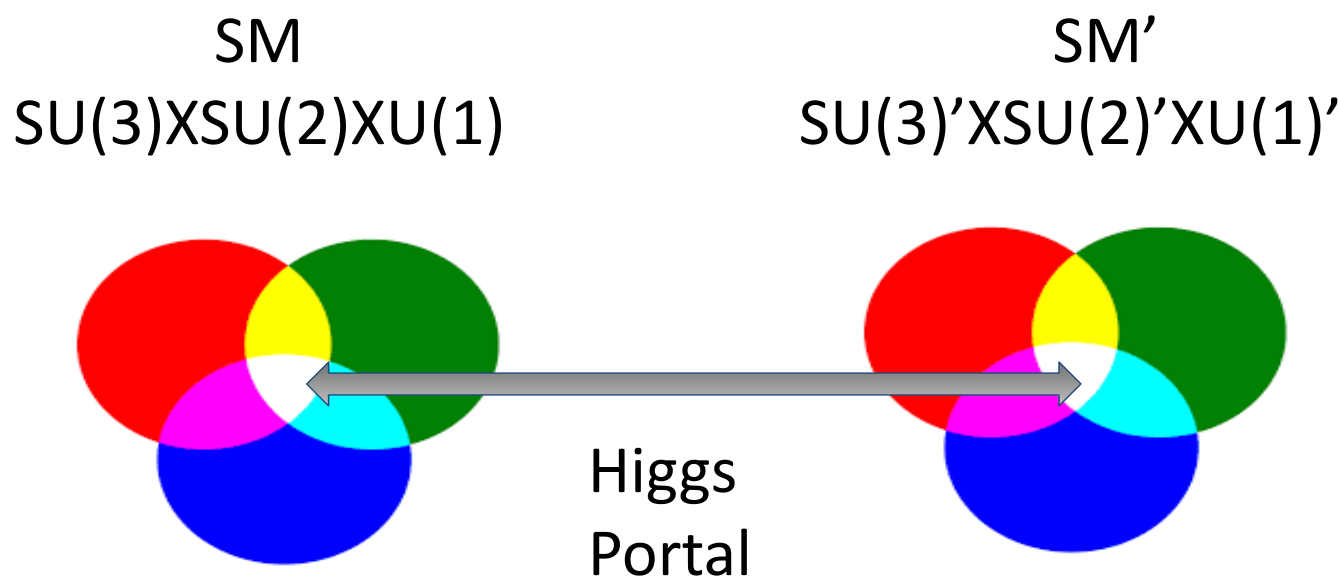
\includegraphics[width=0.87\linewidth]{figs/Portalcartoon.png}
  \caption{A cartoon display of Higgs Portal process}
\end{figure}
BSM mirror QCD scalar glueballs can only decay back to SM particles via Higgs boson decay.

Because of its decay as an off-shell Higgs boson, its cross section is highly suppressed.
The decay branching ratio to the highest mass fermions will be highest following the Yukawa couplings.
The decay ratio into b quarks or $\tau$ leptons is highest depending on the mirror scalar's mass.
However, if the Higgs has leptophilic behavior, the decay ratio into $\tau$ leptons is always the highest.
The displaced decays of the scalars would lead to exotic signatures in CMS, such as distant innermost tracker hits, displaced vertices, and displaced jets.
The phenomenology of long-lived decay increased interest in a neutral naturalness among the particle physics community \cite{Curtin:2015fna,Csaki:2015fba}.
The long-lived scalar model process is shown in Figure \ref{fig:HiggsPortal}.



\begin{figure}[h!]
  \label{fig:HiggsPortal}
  \centering
  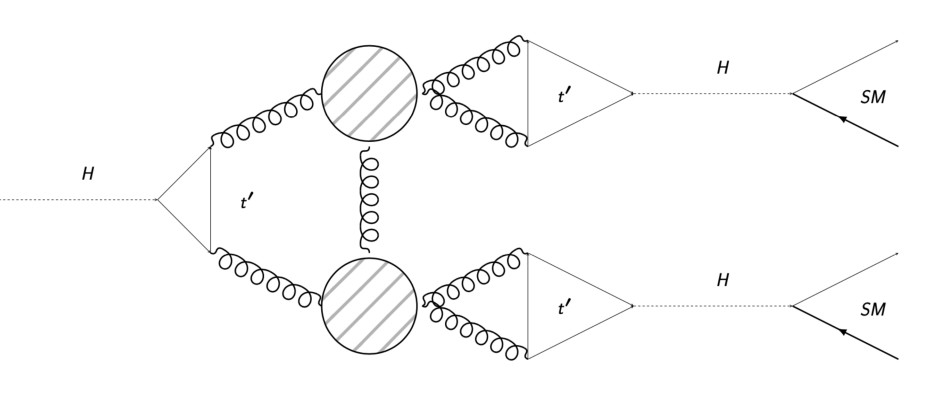
\includegraphics[width=0.87\linewidth]{figs/TwinHiggs.png}
  \caption{A diagram display of Higgs Portal process}
\end{figure}
